%Good alignment of the SVT is critical to achieving the expected tracking performance and physics reach. 
%The sensors must be aligned internally and with respect to the target and other beam line components for optimal performance. 
%The alignment of the test run apparatus proceeds in several steps which must be tied together to achieve the final alignment.
%These include survey measurements of various SVT assemblies, a beam line survey at JLab, and finally 
%a track-based alignment. 

The SVT was aligned using a combination of optical, laser and touch probe surveys at SLAC and JLab. The 
optical survey of individual modules with precision of a few microns are combined with a touch-prove survey 
of the overall SVT support structure, with 25-100 microns precision, to locate the silicon sensor layers with 
respect to the support plates and the mechanical survey balls on the base plate.
After full assembly and installation of the SVT at JLab, a mechanical survey of the SVT base plate position 
inside the pair spectrometer vacuum chamber is used to determine the global position of the SVT with respect 
to CEBAF beam line. 
The resulting survey-based alignment has the position of the silicon sensors correct to within a few hundred 
microns as shown in the mean of the biased track residuals in Fig.~\ref{fig:res_top}.  
\begin{figure*}[]
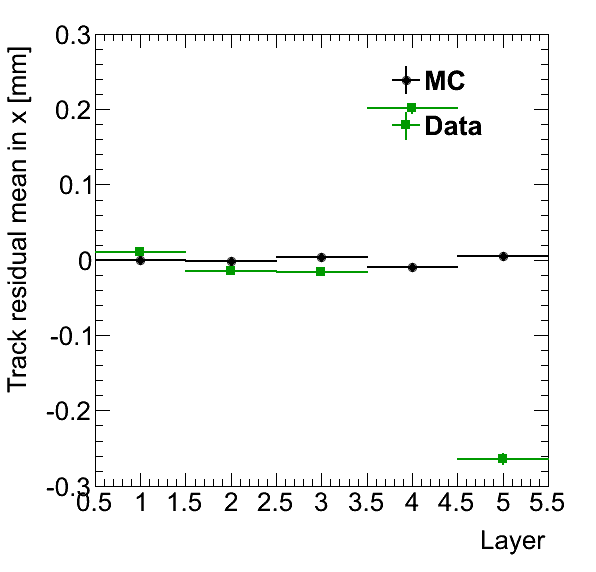
\includegraphics[ scale=0.3]{test2012/alignment/pictures/res_top/h_trk_top_res_y_mean_h_trk_top_res_y_mean_dataMC_trigseltwotrksel4hit_recoilmc_twotrkfilt.png}
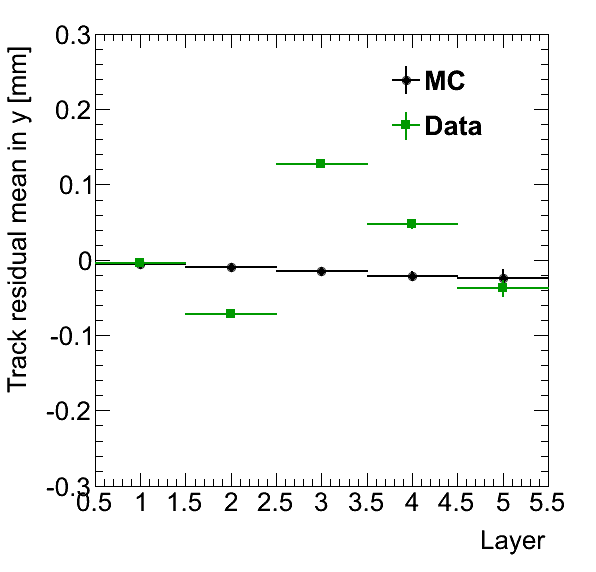
\includegraphics[ scale=0.3]{test2012/alignment/pictures/res_top/h_trk_top_res_z_mean_h_trk_top_res_z_mean_dataMC_trigseltwotrksel4hit_recoilmc_twotrkfilt.png}
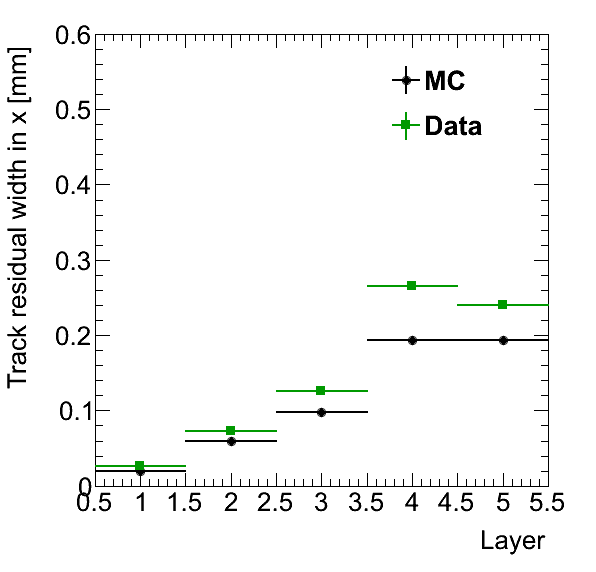
\includegraphics[ scale=0.3]{test2012/alignment/pictures/res_top/h_trk_top_res_y_sigma_h_trk_top_res_y_sigma_dataMC_trigseltwotrksel4hit_recoilmc_twotrkfilt.png}
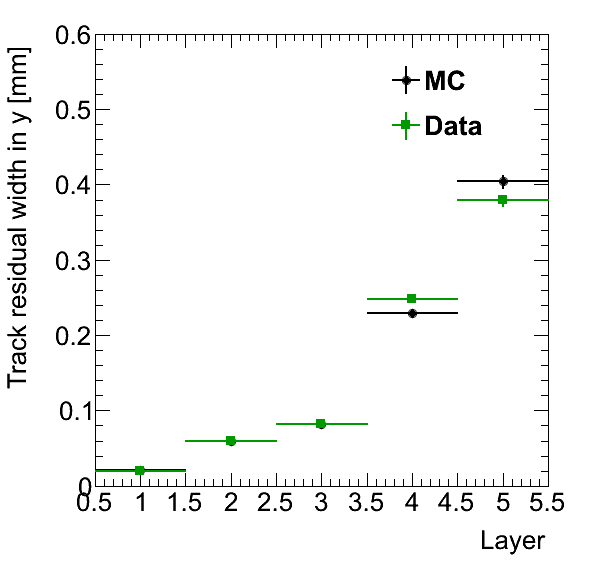
\includegraphics[ scale=0.3]{test2012/alignment/pictures/res_top/h_trk_top_res_z_sigma_h_trk_top_res_z_sigma_dataMC_trigseltwotrksel4hit_recoilmc_twotrkfilt.png}
\caption{\small{Mean (top) and standard deviation (bottom) of biased residuals (i.e. hits are included in the track fit) between the actual hit position and the predicted position from the reconstructed tracks in the bend (left) and non-bend (right) plane in the top half of the SVT after mechanical survey. The smaller width for the 5th layer in the bend plane is an effect from mixing tracks with four or five hit tracks.}}
\label{fig:res_top}
\end{figure*}
The large multiple scattering contribution can be seen by the large increase in the width of the residuals in the later layers. The agreement with simulation is reasonable; a slight track reconstruction algorithm bias can be seen in the mean for the simulation in later layers which will be fixed in the future. 

%In electron running, the beam spot can be used as a constraint in the global track-based alignment. 
We also extrapolate the reconstructed tracks back to the converter located $\approx 77$~cm 
from our first silicon layer to understand the tracker alignment w.r.t. to the other components on the 
beam line. Figure~\ref{fig:extrapol_converter} shows good agreement of the reconstructed track position at the converter with that predicted from simulation using the measured field map of the analyzing magnet to take into account the fringe field. 
\begin{figure*}[t]
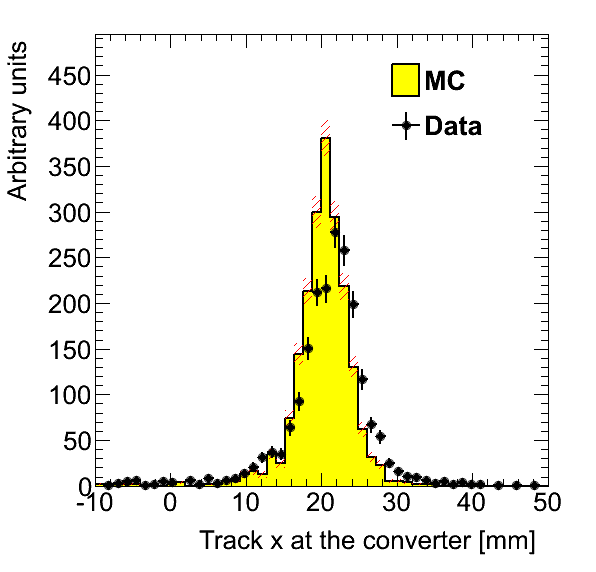
\includegraphics[ scale=0.25]{test2012/alignment/pictures/extrapolation_converter/h_trk_top_fr_conv_y_h_trk_top_conv_y_dataMC_twotrksel.png}
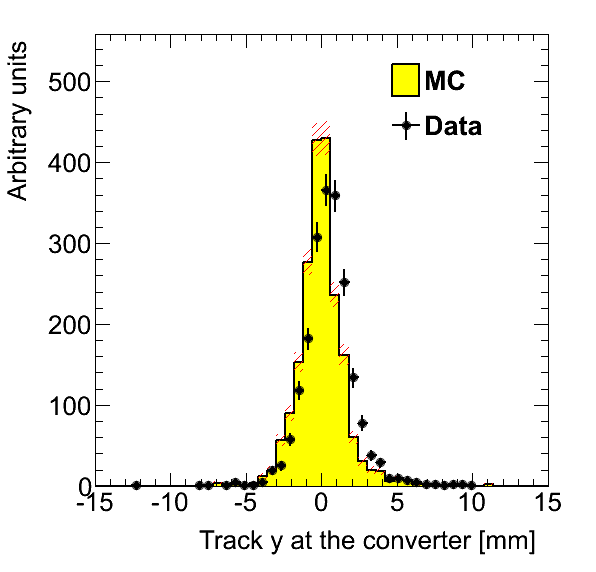
\includegraphics[ scale=0.25]{test2012/alignment/pictures/extrapolation_converter/h_trk_top_fr_conv_z_h_trk_top_conv_z_dataMC_twotrksel.png}
%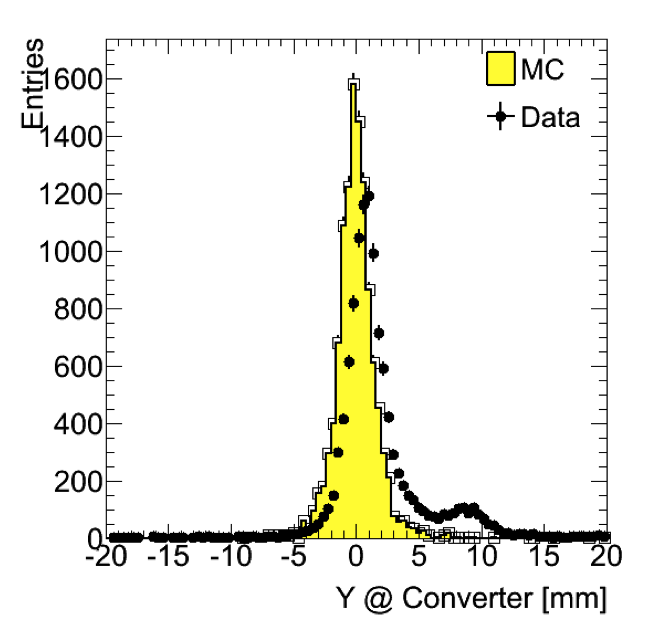
\includegraphics[ scale=0.5]{test2012/alignment/pictures/extrapolation_converter/extrapolation_Y_converter_top.png}
%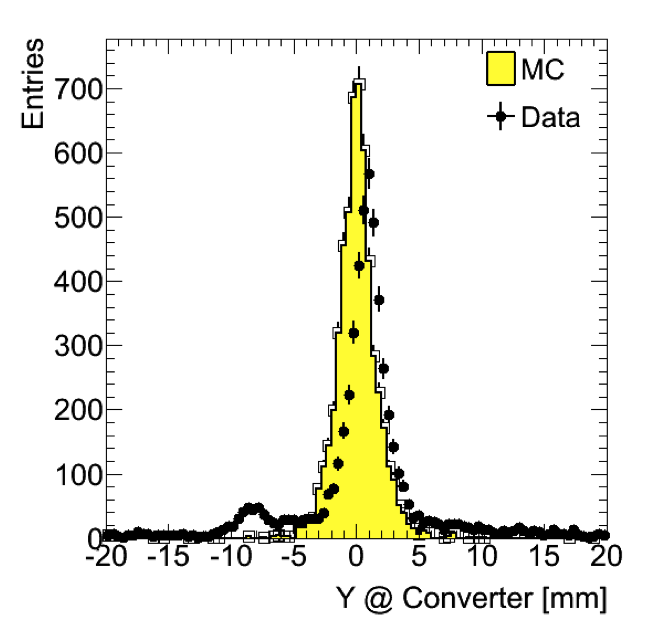
\includegraphics[ scale=0.5]{test2012/alignment/pictures/extrapolation_converter/extrapolation_Y_converter_bot.png}
\caption{\small{Extrapolated track positions for reconstructed e$^{+}$e$^{-}$ pairs in the SVT taking into account the measured fringe field of the analyzing magnet in data and a simulation with ideal geometry.}}
\label{fig:extrapol_converter}
\end{figure*}
The offset of the horizontal position simply reflects the fact that the positions are reconstructed in an SVT-centered coordinate system, which is tilted with respect to the beam coordinate system.
%The width is roughly consistent with between data and simulation with a shift in the bend-plane 
%coordinate for tracks in the bottom half which is likely due to alignment or incomplete description of the 
%magnetic field at the edge of the magnet. 
%There are two small bumps in the vertical position in the data arising from backgrounds 
%originating upstream of the converter verified using the run without a converter.
%The luminous region, inferred from harp scans of the photon beam profile, has a width of about 1~mm 
%%(best described by a double Gaussian: $0.71e^{\frac{x}{0.366}}\times 0.29e^{\frac{x}{1.111}}$)
%and a total beam envelope of around 7~mm. The small bumps in data at $\pm10$~mm 
%are from particles produced upstream of the converter. The width and position of the tracks 
%are roughly consistent with the expected distribution from an ideal geometry as shown by the simulated 
%tracks in the same figures. The larger shift in the bend direction for bottom tracks 
%is still under investigation. 

With initial residuals less than $\sim 500~\mu$m across all layers of 
the tracker and a reconstructed beam profile similar to that expected from simulation, it appears these survey techniques 
are adequate to bootstrap the SVT alignment. 
For HPS, we are developing a more sophisticated global track-based alignment technique to reach 
the final alignment precision. This framework will also enable us to explore and understand important details 
such as weak modes and how dedicated alignment runs 
(e.g. with magnetic field off or with different targets) may shape operational procedures during HPS running.
%Fig.~\ref{fig:test_harpscan} shows a HARP scan taken during the test run. 
%\begin{figure*}[t]
%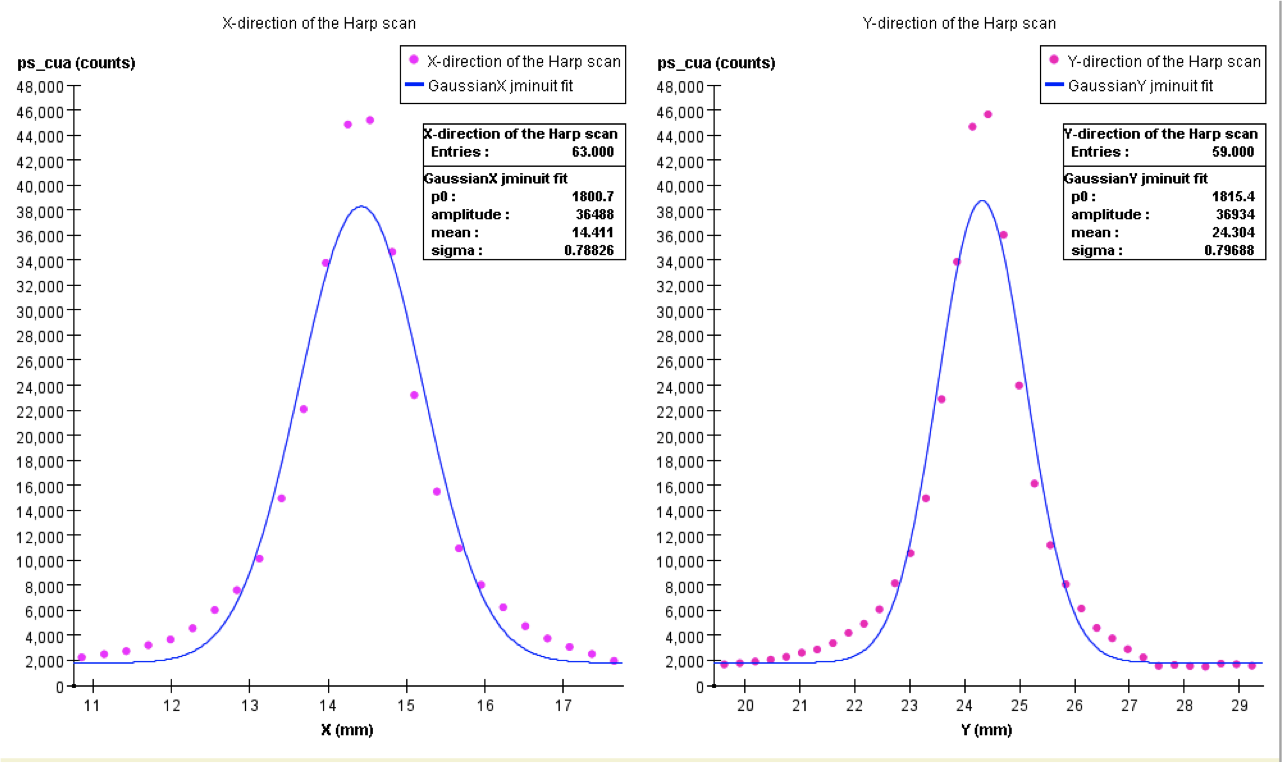
\includegraphics[ scale=0.5]{test2012/alignment/pictures/harp_scan_testrun.png}
%\caption{\small{Photon beam profile HARP scan close to the converter.}}\label{fig:testrun_harpscan}
%\end{figure*}
%The width of the beam can be described by a double Gaussian $0.71e^{\frac{x}{0.366}}\times 0.29e^{1.111}$ which is also used in the simulations. The beam envelope extends out to 
%about 7mm. 
